\documentclass[tikz,border=6pt]{standalone}
\usepackage{amsmath}
\usetikzlibrary{arrows.meta}

\definecolor{metayellow}{RGB}{255,250,181}
\definecolor{stagecyan}{RGB}{185,239,238}
\definecolor{queuegray}{RGB}{214,214,214}
\definecolor{countergreen}{RGB}{218,241,218}

\begin{document}
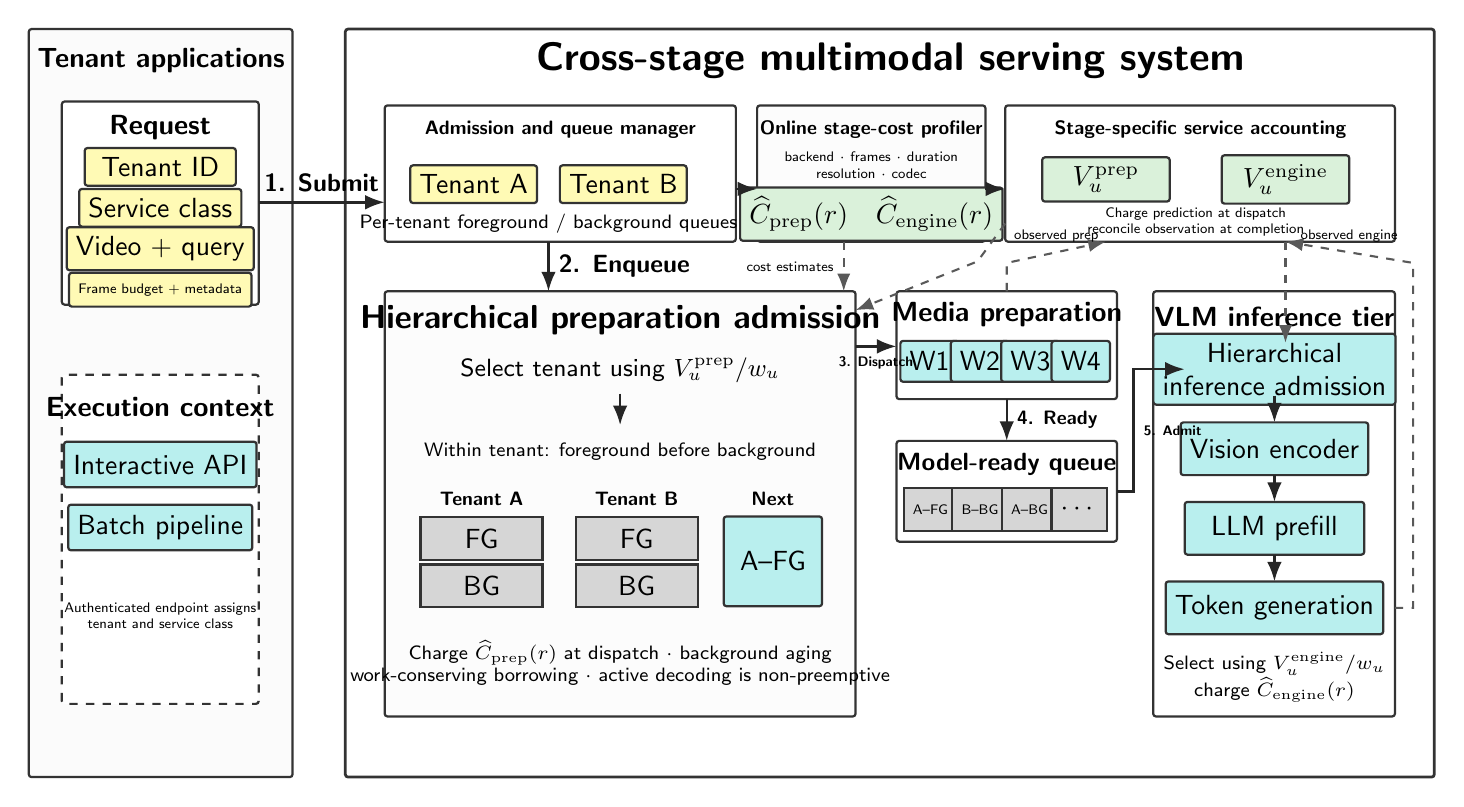
\begin{tikzpicture}[
  font=\sffamily,
  >=Latex,
  line/.style={draw=black!80, line width=0.8pt},
  arrow/.style={->, draw=black!85, line width=0.9pt},
  feedback/.style={->, dashed, draw=black!65, line width=0.75pt},
  panel/.style={line, fill=white, rounded corners=1pt},
  stage/.style={line, fill=stagecyan, rounded corners=1pt, align=center},
  metadata/.style={line, fill=metayellow, rounded corners=1pt, align=center},
  qitem/.style={line, fill=queuegray, minimum height=0.54cm, align=center},
  counter/.style={line, fill=countergreen, rounded corners=1pt, align=center},
  title/.style={font=\bfseries\sffamily}
]

% Tenant applications.
\draw[panel, fill=gray!3] (-0.1,-4.75) rectangle (3.25,4.75);
\node[title, font=\normalsize\bfseries\sffamily] at (1.58,4.35)
  {Tenant applications};
\draw[panel] (0.32,1.25) rectangle (2.82,3.83);
\node[title] at (1.57,3.50) {Request};
\node[metadata, minimum width=1.92cm, minimum height=0.43cm] at (1.57,3.00)
  {Tenant ID};
\node[metadata, minimum width=1.92cm, minimum height=0.43cm] at (1.57,2.48)
  {Service class};
\node[metadata, minimum width=1.92cm, minimum height=0.43cm] at (1.57,1.96)
  {Video + query};
\node[metadata, minimum width=1.92cm, minimum height=0.43cm,
      font=\tiny\sffamily] at (1.57,1.44)
  {Frame budget + metadata};
\draw[panel, dashed] (0.32,-3.82) rectangle (2.82,0.36);
\node[title] at (1.57,-0.05) {Execution context};
\node[stage, minimum width=1.92cm, minimum height=0.58cm] at (1.57,-0.78)
  {Interactive API};
\node[stage, minimum width=1.92cm, minimum height=0.58cm] at (1.57,-1.58)
  {Batch pipeline};
\node[align=center, font=\tiny\sffamily] at (1.57,-2.70)
  {Authenticated endpoint assigns\\tenant and service class};

% Server boundary.
\draw[panel, line width=1pt] (3.92,-4.75) rectangle (17.75,4.75);
\node[title, font=\Large\bfseries\sffamily] at (10.84,4.35)
  {Cross-stage multimodal serving system};

% Admission, profiling, and accounting.
\draw[panel] (4.42,2.05) rectangle (8.88,3.78);
\node[title, font=\scriptsize\bfseries\sffamily] at (6.65,3.47)
  {Admission and queue manager};
\node[metadata, minimum width=1.52cm, minimum height=0.47cm] at (5.55,2.78)
  {Tenant A};
\node[metadata, minimum width=1.52cm, minimum height=0.47cm] at (7.45,2.78)
  {Tenant B};
\node[font=\scriptsize\sffamily] at (6.50,2.28)
  {Per-tenant foreground / background queues};

\draw[panel, fill=gray!2] (9.15,2.05) rectangle (12.05,3.78);
\node[title, font=\scriptsize\bfseries\sffamily] at (10.60,3.47)
  {Online stage-cost profiler};
\node[font=\tiny\sffamily, align=center] at (10.60,3.02)
  {backend $\cdot$ frames $\cdot$ duration\\resolution $\cdot$ codec};
\node[counter, minimum width=2.35cm, minimum height=0.50cm] at (10.60,2.40)
  {$\widehat C_{\mathrm{prep}}(r)\quad
    \widehat C_{\mathrm{engine}}(r)$};

\draw[panel] (12.30,2.05) rectangle (17.25,3.78);
\node[title, font=\scriptsize\bfseries\sffamily] at (14.78,3.47)
  {Stage-specific service accounting};
\node[counter, minimum width=1.62cm, minimum height=0.52cm] at (13.58,2.84)
  {$V_u^{\mathrm{prep}}$};
\node[counter, minimum width=1.62cm, minimum height=0.52cm] at (15.86,2.84)
  {$V_u^{\mathrm{engine}}$};
\node[font=\tiny\sffamily, align=center] at (14.72,2.30)
  {Charge prediction at dispatch\\reconcile observation at completion};

% Hierarchical scheduler.
\draw[panel, fill=gray!2] (4.42,-3.98) rectangle (10.40,1.42);
\node[title, font=\large\bfseries\sffamily] at (7.41,1.05)
  {Hierarchical preparation admission};
\node[font=\small\sffamily] at (7.41,0.42)
  {Select tenant using $V_u^{\mathrm{prep}}/w_u$};
\draw[arrow] (7.41,0.12) -- (7.41,-0.28);
\node[font=\scriptsize\sffamily] at (7.41,-0.62)
  {Within tenant: foreground before background};
\node[font=\scriptsize\bfseries\sffamily] at (5.65,-1.22) {Tenant A};
\node[qitem, minimum width=1.55cm] at (5.65,-1.72) {FG};
\node[qitem, minimum width=1.55cm] at (5.65,-2.32) {BG};
\node[font=\scriptsize\bfseries\sffamily] at (7.62,-1.22) {Tenant B};
\node[qitem, minimum width=1.55cm] at (7.62,-1.72) {FG};
\node[qitem, minimum width=1.55cm] at (7.62,-2.32) {BG};
\node[font=\scriptsize\bfseries\sffamily] at (9.35,-1.22) {Next};
\node[stage, minimum width=1.25cm, minimum height=1.14cm] at (9.35,-2.01)
  {A--FG};
\node[font=\scriptsize\sffamily, align=center] at (7.41,-3.30)
  {Charge $\widehat C_{\mathrm{prep}}(r)$ at dispatch $\cdot$ background aging\\
   work-conserving borrowing $\cdot$ active decoding is non-preemptive};

% Preparation and model-ready queue.
\draw[panel] (10.92,0.05) rectangle (13.72,1.42);
\node[title] at (12.32,1.12) {Media preparation};
\node[stage, minimum width=0.46cm, minimum height=0.52cm] at (11.34,0.53) {W1};
\node[stage, minimum width=0.46cm, minimum height=0.52cm] at (11.98,0.53) {W2};
\node[stage, minimum width=0.46cm, minimum height=0.52cm] at (12.62,0.53) {W3};
\node[stage, minimum width=0.46cm, minimum height=0.52cm] at (13.26,0.53) {W4};

\draw[panel] (10.92,-1.76) rectangle (13.72,-0.48);
\node[title, font=\small\bfseries\sffamily] at (12.32,-0.78)
  {Model-ready queue};
\node[qitem, minimum width=0.55cm, font=\tiny\sffamily] at (11.35,-1.35) {A--FG};
\node[qitem, minimum width=0.55cm, font=\tiny\sffamily] at (11.98,-1.35) {B--BG};
\node[qitem, minimum width=0.55cm, font=\tiny\sffamily] at (12.61,-1.35) {A--BG};
\node[qitem, minimum width=0.48cm] at (13.24,-1.35) {$\cdots$};

% VLM inference tier.
\draw[panel] (14.18,-3.98) rectangle (17.25,1.42);
\node[title] at (15.72,1.10) {VLM inference tier};
\node[stage, minimum width=2.28cm, minimum height=0.67cm] at (15.72,0.43)
  {Hierarchical\\inference admission};
\node[stage, minimum width=2.28cm, minimum height=0.67cm] at (15.72,-0.58)
  {Vision encoder};
\node[stage, minimum width=2.28cm, minimum height=0.67cm] at (15.72,-1.59)
  {LLM prefill};
\node[stage, minimum width=2.28cm, minimum height=0.67cm] at (15.72,-2.60)
  {Token generation};
\node[font=\scriptsize\sffamily, align=center] at (15.72,-3.48)
  {Select using $V_u^{\mathrm{engine}}/w_u$\\
   charge $\widehat C_{\mathrm{engine}}(r)$};

% Numbered data flow.
\draw[arrow] (2.82,2.55) -- node[above, font=\bfseries\small\sffamily]
  {1. Submit} (4.42,2.55);
\draw[arrow] (6.50,2.05) -- node[right, font=\bfseries\small\sffamily]
  {2. Enqueue} (6.50,1.42);
\draw[arrow] (10.40,0.72) -- node[below, font=\bfseries\tiny\sffamily]
  {3. Dispatch} (10.92,0.72);
\draw[arrow] (12.32,0.05) -- node[right, font=\bfseries\scriptsize\sffamily]
  {4. Ready} (12.32,-0.48);
\draw[arrow] (13.72,-1.12) -- (13.93,-1.12) --
  node[right, font=\bfseries\tiny\sffamily] {5. Admit}
  (13.93,0.43) -- (14.58,0.43);
\draw[arrow] (15.72,0.095) -- (15.72,-0.245);
\draw[arrow] (15.72,-0.915) -- (15.72,-1.255);
\draw[arrow] (15.72,-1.925) -- (15.72,-2.265);

% Metadata, predictions, accounting, and observed-service feedback.
\draw[arrow] (8.88,2.72) -- (9.15,2.72);
\draw[arrow] (12.05,2.72) -- (12.30,2.72);
\draw[feedback] (10.25,2.05) -- node[left, font=\tiny\sffamily]
  {cost estimates} (10.25,1.42);
\draw[feedback] (12.32,1.42) -- (12.32,1.78) --
  node[above, font=\tiny\sffamily] {observed prep} (13.58,2.05);
\draw[feedback] (17.25,-2.60) -- (17.48,-2.60) --
  (17.48,1.78) -- node[above, font=\tiny\sffamily]
  {observed engine} (15.86,2.05);
\draw[feedback] (12.30,2.28) -- (11.95,1.80) -- (10.40,1.18);
\draw[feedback] (15.86,2.05) -- (15.86,0.765);

\end{tikzpicture}
\end{document}
